\documentclass[output=paper]{langscibook}
\ChapterDOI{10.5281/zenodo.15148196}
\author{Marijn van 't Veer\orcid{0000-0003-3415-7199}\affiliation{Leiden University; University of Amsterdam} and         Martine Bruil\orcid{}\affiliation{Leiden University} and        Oleksandra Damonte-Matveienko\orcid{}\affiliation{Leiden University}}
\title{Pre-aspiration in Ecuadorian Siona}
\abstract{Ecuadorian Siona (Tukanoan) has been put forth as a language which potentially manifests pre-aspiration \citep{Bruil:2014}, but the phonemic status of voiceless pre-aspirated obstruents in the language has, as of yet, not been established. Earlier analyses of related languages have proposed an analysis in terms of vowel devoicing \citep[90]{Wheeler:1987a}, but we propose that a consonantal analysis is superior. In this study we examine the distribution of pre-consonantal [h] in Ecuadorian Siona, and conclude that it is best analyzed as the result of a prosodically driven enhancement process which causes pre-aspiration of non-laryngealized obstruents in foot-head onsets.
\keywords{Ecuadorian Siona, Tukanoan, pre-aspiration, prosody, foot structure}}

\begin{document}

\maketitle


\section{Introduction}\label{sec-intro}
Ecuadorian Siona (sion1247) is a Western Tukanoan language, spoken in the North East of Ecuador (\cite{Bruil:2014}; see \figref{fig-villages} below). A quite common phonological phenomenon in Tukanoan languages is pre-aspiration (see, for example, \citealt{Stenzel:2007}, on Kotiria). In Ecuadorian Siona, too, a pre-consonantal glottal fricative occurs frequently. However, as noted in \citet{Bruil:2014}, there are certain complicating factors that mean an analysis of pre-consonantal [h] in Ecuadorian Siona as pre-aspiration is not straightforward.

In this study, we closely examine the occurrence of pre-consonantal [h] in light of three alternative analyses. First, since \mbox{/h/} freely occurs in onsets, we consider that the segment has a phonemic, consonantal status, also in pre-consonantal positions. This analysis is rejected on the basis of the predictability of pre-con\-so\-nan\-tal [h]. Then, we analyze pre-aspiration as the result of phonological processes. We first consider the coda epenthesis hypothesis first, but find that it is inadequate in certain respects. We then turn to the pre-aspiration hypothesis, and argue that this is the best analysis: not only do its predictions correspond to the observed facts, but it is also motivated in terms of prosodic strength. We conclude the chapter with a diachronic overview of pre-aspiration in Ecuadorian Siona and in its Tukanoan cognate languages.

The chapter is organized as follows. In \sectref{sec-preasp} we investigate the typology, phonetics and phonology, and genesis of pre-aspiration, before turning to the synchronic and diachronic analyses in \sectref{sec-analysis}, while \sectref{sec-conc} presents some concluding remarks. First, however, we briefly provide an overview of some general characteristics of Ecuadorian Siona (\sectref{sec-LangBG}), and the conventions we adopt in representing the data (\sectref{conv}).\footnote{Parts of this study are built on the third author's undergraduate thesis, completed in 2021 under the supervision of the first two authors, at the University of Amsterdam.}


\subsection{Language background}\label{sec-LangBG}
\largerpage
Ecuadorian Siona is a Western Tukanoan language, closely related to Sekoya (seco1241) and Colombian Siona, spoken in the rural areas of the Sucumb\'ios province of Eastern Ecuador. Most of the speakers live in seven Siona villages: Puerto Bol\'ivar, San Victoriano, Tarab\"eaya, Sototsiaya, Orahu\"eaya, Aboqu\"ehuira and Bi'aña. A publication on Ecuador's indigenous languages from 2001 estimates the number of Siona speakers to be between 200 and 250 \citep{Mejeant:2001}. A more recent, albeit  informal survey (conducted by the second author together with the community members in 2016), established a number of roughly 300 speakers. This means that the language is severely endangered. The data reported in the current study are based on fieldwork performed by the second author in 2010--2015 \citep{Bruil:2014}, in the Puerto Bol\'ivar and Sototsiaya villages (see \figref{fig-villages}). The Siona people refer to themselves as \textit{bãĩ}, which means `people', and to their language as \textit{bãĩkoka} `the language of the people'.


\begin{figure}
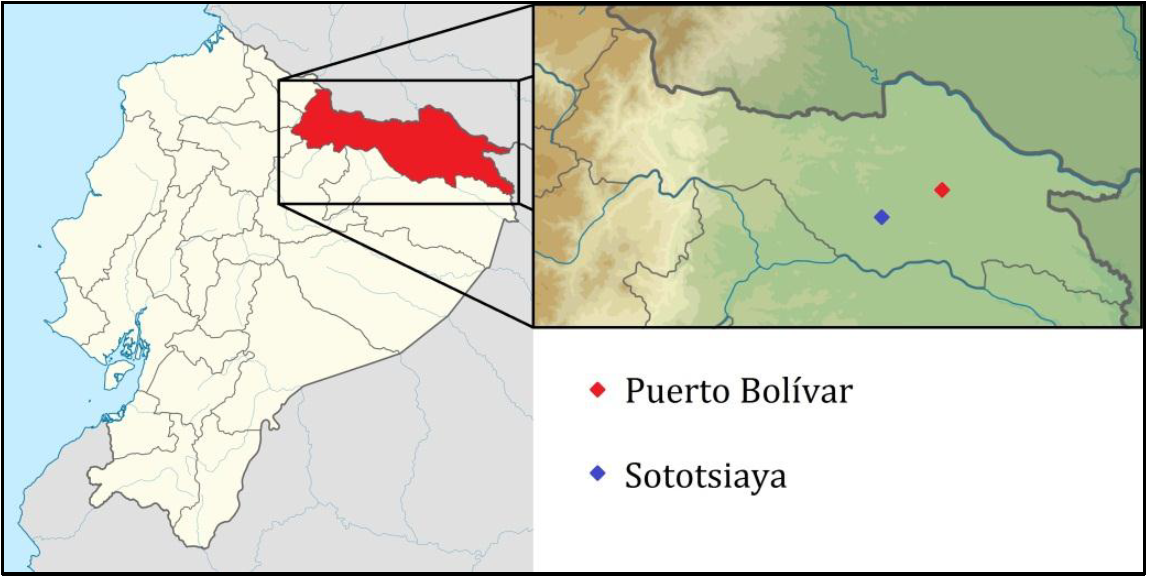
\includegraphics[height=.3\textheight]{figures/Picture1.png}
\caption{Map of the fieldwork sites (adapted from \citealt[5]{Bruil:2014})}
\label{fig-villages}
\end{figure}


A number of classifications have been proposed for the Tukanoan language family; here, we adopt the one by \citet{Chacon:2014}, with an additional distinction between Ecuadorian Siona and Colombian Siona \citep[11]{Bruil:2014}. In Chacon's classification, Tukanoan branches into two major subgroups: Western Tukanoan and Eastern Tukanoan. Whereas the latter is further subdivided into Southern, Western, and Eastern, the former is proposed to be a single group, consisting of the languages Kueretu (cure1236), M\'aih\'iki (orej1242), Koreguaje (kore1283), Sekoya, and Siona \citep{Chacon:2014}. 

Earlier studies on Siona have focused on the Colombian variety \citep{Wheeler:1967, Wheeler:1970, Wheeler:1987a, Wheeler:1987b, Wheeler:2000, WheelerWheeler:1975}, but the Ecuadorian variant differs considerably from it in phonological, lexical and morphosyntactic aspects. In fact, Ecuadorian Siona is in some ways more similar to (closely related) Sekoya than to Colombian Siona. For example, unlike Colombian Siona, both Ecuadorian Siona and Sekoya lost the word-internal voiced velar stop. On the other hand, Ecuadorian Siona shows a type of vowel assimilation that is absent in both Colombian Siona and Sekoya  (see \citealt[10--12]{Bruil:2014}, for a more detailed discussion). Therefore, \citet{Bruil:2014} proposes that the two varieties of Siona, together with Sekoya, can be seen as a tripartite dialect continuum.

\subsection{A brief sketch of Ecuadorian Siona phonology}\label{sec-phonBG}

\subsubsection{Phoneme inventory}
The consonantal inventory of Ecuadorian Siona is given in \tabref{tab-cons}.  The coronals [d, ɾ] are not included in \tabref{tab-cons}, as their status as potential allophonic variants of \mbox{/t̰/} is a topic currently under investigation (see also \tabref{tab-allophon}). \figref{tab-vow} presents the Siona vowel system, which has six contrastive vowel qualities and in addition, nasality as a distinctive feature (transcribed with a tilde above the vowel). Contrary to many other Tukanoan languages, Ecuadorian Siona has phonemic nasal consonants and nasal vowels \citep{BruilStewart:2022}. Underlyingly, there is no length contrast for vowels, but long vowels may appear in some surface forms. This is due either to a number of active vowel coalescence processes \citep[115--117]{Bruil:2014}, or lengthening due to the bimoraic stem constraint (see \sectref{sec-supra}).

\begin{table}
\begin{tabular}{lcccccc}
    \lsptoprule
&	Labial	&	Coronal	&	\multicolumn{2}{c}{Dorsal}				& \multicolumn{2}{c}{Laryngeal}\\\cmidrule(lr){4-5}\cmidrule(lr){6-7}
&			&			&	Plain		&	Lab.				&		Plain		&	Lab.	\\ \midrule
Plosives & \\
\quad Plain			&	p		&	t		&	k		&	kʷ		&			\\
\quad Lar.	&	p̰	&	t̰	&	k̰	&	k̰ʷ&	ʔ	&	\\
Affricates	&			&	ʧ		&			&						&			\\
Fricatives	& \\
\quad Plain			&			&	s		&			&						&	h	&  hʷ	\\
\quad Lar.	&			&	s̰	&			&						&			\\
Nasals	& \\
\quad Plain			&	m		&	n		&			&						&			\\
Approximants			&			&	j		&			&	w					&			\\
\lspbottomrule
\end{tabular}
\caption{Consonants of Ecuadorian Siona (adapted from \citealt[87]{Bruil:2014} and  \citealt{BruilStewart:2022})}\label{tab-cons}
\end{table}

\begin{figure}[ht]
	\centering
	{\large
	\begin{vowel}[three]
		\putcvowel[l]{i}{1}
		\putcvowel[r]{\~{i}}{1}	
		\putcvowel[l]{e}{2}
		\putcvowel[r]{\~{e}}{2}		
		\putcvowel[l]{a}{4}
		\putcvowel[r]{\~{a}}{4}		
		\putcvowel[l]{ɨ}{9}
		\putcvowel[r]{\~{ɨ}}{9}		
		\putcvowel[l]{u}{8}
		\putcvowel[r]{\~{u}}{8}		
		\putcvowel[l]{i}{1}
		\putcvowel[r]{\~{i}}{1}		
		\putcvowel[l]{o}{7}
		\putcvowel[r]{\~{o}}{7}		
	\end{vowel}}\caption{Vowels of Ecuadorian Siona}\label{tab-vow}
\end{figure}


\subsubsection{Laryngeality}\label{sec-laryng}
\tabref{tab-cons} shows that Ecuadorian Siona contrasts obstruents not in terms of voiced and voiceless, but rather in terms of plain and laryngealized. The non-glottal obstruent system displays near-perfect symmetry in terms of this contrast (only the affricate \mbox{/ʧ/} lacks a laryngealized counterpart). An in-depth study on the phonetics of laryngealized obstruents is still lacking. However, based on the preliminary analysis in \citet{Bruil:2014}, we can make a number of observations.
% \footnote{The attentive reader may note that the undertildes used to indicate laryngeality are not centered under the consonant, nor under the vowel, in the examples in \tabref{tab-lar}. This is a deliberate choice, to express the phonetic reality that vowels following laryngealized consonants are partially realized with creaky voice.}

\largerpage
First of all, there are four laryngealized stops: /p̰, t̰, k̰, k̰ʷ/. All of these may occur word-initially, but only the first two are allowed in other positions (i.e., intervocalically).\footnote{The dorsal laryngealized stops \mbox{/k̰, k̰ʷ/} can be found in intervocalic positions, but only in the context of compounds, the phonological interpretation of which is uncertain for now.} The realization of the laryngealized stops is variable, but generally predictable: in word-initial position, laryngealization is realized as creak, with its partial spreading as creaky voice onto the following vowel. Intervocalically, \mbox{/p̰, t̰/} are realized as sonorant-like [β, ɾ] respectively (see \citealt[93--95]{Bruil:2014} for more details on this allophonic relationship).\footnote{See also \citet{BotmaVeer:2013} for an analysis of intervocalic voicing as weakening, which is especially pertinent in combination with \citet{GolstonKehrein:2015}'s proposal for the relative sonority of laryngeals.} \tabref{tab-lar} provides examples of the four stops in various positions. For the coronal \mbox{/t̰/}, the range of allophonic realizations in different morphophonological positions is more varied (e.g., it can be realized as [d], as indicated in \tabref{tab-allophon}), but an in-depth discussion of this is beyond the scope of the current chapter. A preliminary sketch can be found in \citet{Bruil:2014}, and more research is currently underway.

\begin{table}\centering
\begin{tabular}{llll}\lsptoprule
		&	Word-initial	&	Word-internal	&	Suffix-initial	\\ \midrule
/p̰/	&	[p̰eo.je]	&	[ho.βo]		&	[wɨo-βi]	\\
		&	`to not be/have'	&	`the middle'	&	`he began'	\\
/t̰/	&	[t̰ai.je]	&	[we.ɾo.je]	&	[ho-ɾo]		\\
		&	`to come'		&	`to buy'		&	`flower'		\\
/k̰/	&	[k̰o.he]	&				&				\\
		&	`hole'		&				&				\\
/k̰ʷ/	&	[k̰ʷiː.je]	&		&				\\
		&	`to scream'	&				&				\\ \lspbottomrule				
\end{tabular}\caption{Positional variants of laryngealized stops (from \citealt[93]{Bruil:2014})}\label{tab-lar}
\end{table}

Next, the laryngealized sibilant \mbox{/s̰/} is similar to the laryngealized dorsal stops in terms of distribution: it only occurs in word-initial position. Unlike in the case of the laryngeal dorsals, however, laryngealization is lost when /s̰/ appears as the first segment of a non-initial member of a compound, in which case the contrast between /s/ and /s̰/ is neutralized (in favour of /s/). Finally, both /s/ and /s̰/ are subject to optional but frequent affrication, by which they change into affricates [t͡s] and [t͡s̰] respectively (examples from \citealt[100]{Bruil:2014}):\footnote{The phonetic transcriptions throughout this chapter are presented in and adapted according to IPA. More conventions, specifically pertaining to Siona examples, are discussed in \sectref{conv}.}

\begin{exe}
\ex\label{exe-lar-sibfort}
\begin{xlist}
	\ex {[}sai.je] $\sim$ [tsai.je]\\`to go'
	\ex {[}$\undertilde{\mathrm{si}}$a.ja] $\sim$ [$\undertilde{\mathrm{tsi}}$a.ja]\\`river'
\end{xlist}
\end{exe}

In \sectref{sec-glotphon} below, we consider the phonemic status of /h/ in relation to pre-aspiration in more depth. However, some remarks regarding the glottal stop in Ecuadorian Siona are necessary here. Phonologically, it stands apart from the other consonants by being barred from word-initial position.\footnote{\citet[95]{Bruil:2014} notes that the glottal stop may be epenthesized in word-initial position, but is never contrastive there.} In intervocalic position, it is contrastive, and apart from the issue of pre-consonantal /h/, it is the only consonant that may occur in word-internal codas. In terms of articulation, \citet{Bruil:2014} notes that the glottal stop rarely causes full occlusion, and in intervocalic position, is often realized as a period of creaky voice in the vowel. 

\subsection{Laryngeal segments}
In this section, we briefly introduce the status of the glottal fricative, which is phonemic in onset positions and, we argue, non-phonemic in pre-consonantal positions. Although the glottal stop is by no means the focus of the current chapter, its close affinity to the glottal fricative (both in its phonetic content and in its distributional properties) prompts us to briefly discuss it below, in \sectref{sec-glotstop}.

\subsubsection{The status of the glottal fricative}\label{sec-glotphon}
As seen in \tabref{tab-cons} above, the glottal fricative /h/ is part of the underlying phonemic inventory of Ecuadorian Siona. An important argument for the phonemic status of /h/ is that it is not \emph{restricted} to pre-consonantal position. It occurs in onsets, too: both in word-initial (\ref{ex-honset-word}), root-internal (\ref{ex-honset-stem}), and suffix-initial (\ref{ex-honset-suff}) contexts (adapted from \citealt[102]{Bruil:2014}):

{\multicolsep=0pt\begin{exe}
\ex\label{exe-honset}
\begin{xlist}
\begin{multicols}{3}
\ex\label{ex-honset-word} Word-initial:\\
\glll [{hɨo.je}]\\
/{hɨo-je}/\\
slash-\textsc{clf.gen}\\
\trans `to slash'
\ex\label{ex-honset-stem} Root-internal:\\
\glll [jaʔ.hi.je]	\\
/jaʔhi-je/ \\
ripen-\textsc{clf.gen}\\
\trans `to ripen'
\ex\label{ex-honset-suff}Suffix-initial:\\
\glll [kaː.hi]	\\
/kaː-hi/	\\
say-\textsc{3s.m.prs.ass}\\
\trans `he says'
\end{multicols}
\end{xlist}
\end{exe}}

Examples of words presenting difficulty in determining the status (or affiliation) of [h] are given in (\ref{exe-hcoda-parse}).\footnote{Examples from  \citep[102]{Bruil:2014}. Note that trisyllabic [ahpasi] `sapote' is a rare exception to the bimoraic stem constraint, potentially due to it being a loanword. Some other examples exist, see for instance footnote 97 in \citet[148]{Bruil:2014} for animal names that consist of three moras and that appear to be historically multi-morphemic.}

\begin{exe}
\ex\label{exe-hcoda-parse}
\begin{xlist}%\multicolsep=0pt
% \begin{multicols}{2}\raggedcolumns
\ex
\glll [ah.pa.si]\\
ahpasi\\
sapote\\
\trans `sapote (fruit sp.)'
\ex
\glll [soh.to]\\
sohto\\
clay\\
\trans `clay'
\ex
\glll [ah.ʧa.je]\\
ahʧa-je\\
listen-\textsc{clf.gen}\\
\trans `to listen'%\columnbreak
\ex
\glll [nãh̃.so]\\
nahso\\
wooly.monkey\\
\trans `wooly monkey (monkey sp.)'
\ex
\glll [p̰ah.ku]\\
p̰ah.ku\\
pomfret\\
\trans `pomfret (fish sp.)'
% \end{multicols}
\end{xlist}
\end{exe}

The main question, thus, is how to decide on the status of the glottal fricative in such cases, and how to best analyze such a status phonologically. The matter of coda-h versus pre-aspiration in Ecuadorian Siona was first identified in \citet[102--106]{Bruil:2014}, and is further taken up in the current study in \sectref{sec-analysis}.

The initial analysis of pre-aspiration in Ecuadorian Siona made a distinction between root-internal and root-external cases \citep{Bruil:2014}. In our analysis, we argue that such a distinction is only a secondary effect of the smaller distributional freedom that suffixes enjoy when it comes to consonants. One important argument that was given in support of this dichotomy is the apparent difference in the distribution of pre-consonantal [h]. Inside roots, it may only occur before non-laryngealised obstruents, but outside roots, and in a limited number of cases, it may also precede [ɲ]. In our current analysis, we propose that this difference is only superficial, and that careful inspection of the different phonological processes at work reveals that underlyingly, there is no fundamental difference in the distribution of pre-consonantal [h] between root-internal and root-external cases. Secondly, in her initial exploration of Ecuadorian Siona pre-aspiration, \citet{Bruil:2014} proposes that in root-external position, pre-aspiration only occurs at morpheme boundaries. This observation would suggest that pre-aspiration would be sensitive to morphological structure beyond the distinction between root-level phonology and word-level phonology. However, on closer inspection, we propose that regardless of morphological context, pre-aspiration is still a prosodic process. Most, if not virtually all, suffixes in Ecuadorian Siona are monosyllabic, rendering the morpheme boundary approach and the prosodic approach to largely make identical predictions.\footnote{There is one bisyllabic suffix [wesɨ] `for ever', and on close inspection, the second consonant [s] does indeed receive some pre-aspiration.} Since the root-internal versus root-external cases are superficially different, however, we will use the distinction to guide the discussion of data below in \sectref{sec-desc}.


\subsubsection{The matter of the glottal stop}\label{sec-glotstop}
One of the major issues that we have not addressed specifically in this chapter is the fact that pre-consonantal [h] is not the only laryngeal that can occur post-vocalically in Ecuadorian Siona: so can [ʔ]. In fact, \citet{Bruil:2014} proposes that  [h] and [ʔ] constitute the only consonants that may occur in codas.


In this study, we have argued that this is not the case, at least for [h]; rather, when it occurs pre-consonantally, it is better analyzed as a case of pre-aspiration. This begs the question of whether Ecuadorian Siona allows for codas at all, since in that case, only one segment (the glottal stop) may occur in that position. On the one hand, it is tempting to group both [h] and [ʔ] in one and the same group, based on their apparent positional distribution (although we now know that this is not correct) but also based on them being the only (bare) laryngeals in the language.\footnote{Bare, as opposed to the laryngealized consonants.} There are important differences, however, not least of which is that [h] can readily occur in onset positions and hence must be phonemic /h/ there.

The distribution of of the glottal stop in Tukanoan languages in general is special, however, to the degree that it has been proposed to be a ``suprasegmental'' feature, which is not directly attached to a skeletal slot but rather to a higher order constituent in the prosodic hierarchy.

This is precisely the analysis put forward by \citet{Stenzel:2007} with regard to Kotiria (guan1269). While not predictable, there is good evidence to consider the glottal stop not as a ``regular'' phoneme in the language, but rather as a moraic dependent, to be syllabified as necessitated by the morphophonological context. One particularly strong argument is that the glottal stop in Kotiria displays a degree of independence that is typical of suprasegmental features, such as tone or nasality in some cases of nasal harmony.

Kotiria is not Ecuadorian Siona, however, so we cannot blindly adapt the suprasegmental analysis of the glottal stop here. For one thing, there is no tone in Ecuadorian Siona, and thus no interactions between glottalisation and tone either. A further difference between the assignment of the glottal stop in Kotiria and Ecuadorian Siona is that in Kotiria glottal stops generally only occur in the root, whereas in Siona they are also found in suffixes. Finally, pre-aspiration is more complex in Ecuadorian Siona, primarily because of the root-truncation process that we have seen interacts with pre-aspiration.

However, we are sympathetic to the idea of a suprasegmental glottal stop, and there is good reason to assume that it is, indeed, a viable avenue of further research in Ecuadorian Siona. Importantly, a prediction of such an analysis, in combination with our prosodic analysis of Ecuadorian Siona pre-aspiration, is that we would not expect to see the two phenomena occur simultaneously. In other words, words of the form [CV.\textsuperscript{ʔh}CV] are predicted to be ungrammatical. \citet{Stenzel:2007} shows that this prediction is borne out in Kotiria, and in (\ref{exe-gs-h-nogood}) we see that in Ecuadorian Siona, too, no such words exist.

\begin{exe}
\ex\label{exe-gs-h-nogood}
\begin{xlist}
% a
\ex
% \begin{multicols}{2}
	\ea
	\glll [ah.pa.si]\\
	ahpasi\\
	sapote\\
	\trans `sapote'\\
	{\citep[102]{Bruil:2014}}
	\ex \glll [pũʔ.pu.je]\\
	pũʔpu-je\\
	smoke-\textsc{clf:gen}\\
	\trans `to smoke'\\
	{\citep[90]{Bruil:2014}}
	\z
% \end{multicols}
% b
\ex
% \begin{multicols}{2}
	\ea
	\gll [wah.ti]\\
	wahti\\
	\trans `bad spirit'\\
	{\citep[84]{Bruil:2014}}
	\ex \gll [waʔ.ti]\\
	waʔti\\
	\trans `machete'\\
	{\citep[84]{Bruil:2014}}
	\z
% \end{multicols}
% c
\ex
% \begin{multicols}{2}
	\ea
	\gll [p̰õh̃.sa]\\
	bõhsa\\
	\trans `achiote'\\
	{\citep[20120912elicr007]{Bruil:2012}}
	\ex
	\gll [mõʔ.se]\\
	mõʔse\\
	\trans `day'\\
	{\citep[20120919elicr005]{Bruil:2012}}
	\z
% \end{multicols}
% d
\ex
% \begin{multicols}{2}
	\ea
	\glll [kah.kao.ɲã]\\
	kahka-o-jã\\
	enter-\textsc{2/3s.f.pst.n.ass-rep}\\
	\trans `You (\textsc{f})/she entered, they say'\\
	{\citep[20120918elicr003]{Bruil:2012}}
	\ex \glll [ʧaʔ.kao.ɲã]\\
	ʧaʔka-o-jã\\
	jump-\textsc{2/3s.f.pst.n.ass-rep}\\
	\trans `You (\textsc{f})/she jumped, they say'\\
	{\citep[20120918elicr003]{Bruil:2012}}
	\z
% \end{multicols}
% e
\ex
% \begin{multicols}{2}
	\ea
	\glll [ĩh̃.ɲõ]\\
	ĩhjõ\\
	here\\
	\trans `here'\\
	{\citep[20120912elicr007]{Bruil:2012}}

	\ex \glll [mãʔ.ɲõ.ko]\\
	maʔjõ-ko\\
	star-\textsc{clf:anim.f}\\
	\trans `star'\\
	{\citep[20120919elicr005]{Bruil:2012}}
	\z
% \end{multicols}
\end{xlist}
\end{exe}

At first glance, then, it looks like the suprasegmental analysis of the glottal stop and the prosodic analysis of pre-aspiration complement each other well, but we cannot provide a conclusive synthesis within the scope of the current study.





\subsection{Suprasegmental structures}\label{sec-supra}
Our analysis of pre-aspiration in Ecuadorian Siona below leans heavily on prosodic constituents. Before we proceed with the analysis (in \sectref{sec-analysis}), let us briefly consider the structure of syllables and feet in the language.

Syllables in Ecuadorian Siona consist of a (vocalic) nucleus, either simplex or branching, an optional onset, and an optional post-nuclear rhyme (coda), which may only be occupied by glottal consonants \citep[83--84]{Bruil:2014}. In other words, the \emph{surface} syllable template appears to be (C)V(V/H).\footnote{Where ``H'' stands for either of the two laryngeals [ʔ, h].} Branching nuclei may be either long vowels (\ref{ex-longV}) or diphthongs (\ref{ex-diph}); in both cases, the nucleus projects two moras (examples adapted from \citealt[84--85]{Bruil:2014}).\footnote{In our description and analysis, we take the mora to be an abstract unit of quantity for non-onset segments, that plays a role in, for example, maximal stem size. Typologically, moras can potentially be associated with any vowel or consonant that is not in an onset. In the case of Ecuadorian Siona, we argue that only vowels are associated with a mora. Since an in-depth analysis of the prosodic properties of Ecuadorian Siona currently does not exist, we cannot yet stipulate whether moras play a role in, for example, stress assignment. For an in-depth exploration of the role of moras in language, see \citet{Hayes:1989, Hayes:1995}.} The rhyme may maximally dominate two segmental positions, but we argue below that codas are not moraic (\ref{ex-coda}).\footnote{Example adapted from \citet[149]{Bruil:2014}.} In fact, the representations in (\ref{exe-sylls}) should be taken as surface descriptions exclusively, since we argue below that pre-consonantal [h] is not a coda at all. Furthermore, we have reasons to believe that assigning the glottal stop to a coda position is also not as straightforward as it may initially seem (see \sectref{sec-glotstop}). Finally, codas are not allowed in word-final syllables.\footnote{An exception is made for borrowings such as [moh.tor] `motor' from Spanish \citep[84]{Bruil:2014}.}


\begin{exe}
\columnsep=-4pt
\begin{multicols}{3}
\ex\label{exe-sylls}	\begin{xlist}
		\ex\label{ex-longV} 
		\begin{forest}
			[σ
			  [k, tier=lowest]
			  [µ [a, tier=lowest, name=a] ] 
			  [µ, name=mu]
			]
	    \draw (a.north) -- (mu.south);
		\end{forest}\\
		\gll kaː- \\
        say\\
        \trans `to say'
        
		\ex\label{ex-diph}
		\begin{forest}
		  [σ
		    [s,tier=lowest]
		    [µ [a,tier=lowest] ]
		    [µ [o,tier=lowest] ]
		  ]
		\end{forest}\\
        \gll sa-o- \\
        go-\textsc{caus}\\
        \trans `to let go'
        
		\ex\label{ex-coda}
		\begin{forest}
		[,phantom
		  [σ
		    [w, tier=lowest]
		    [µ [a, tier=lowest]]
		    [h, tier=lowest]
		  ]
		  [σ, calign=child, calign child=2
		    [t, tier=lowest]
		    [µ [i,tier=lowest]]
		  ]
		]
		\end{forest}\\
        \gll wahti \\
        bad.spirit\\
        \trans `bad spirit'
	\end{xlist}
\end{multicols}
\end{exe}


Even if we accept that both laryngeal sounds can occupy coda position, this does not automatically entail moraicity; languages may associate moras with vowels, but not with codas (see \citealt{GordonETAL:2008} for an overview of this typology). An argument for this is an observation that, much like other Tukanoan languages, such as Barasana (bara1380), Tatuyo (tatu1247), Kotiria \citep[85--86]{Bruil:2014}, and Tukano (tuca1252) \citep{Ramirez:1997}, Ecuadorian Siona abides by what can be described as a bimoraic stem constraint. This implies that stems must contain at least \emph{and} at most two moras. Stems may consist of a bare root, or a root followed by no more than one derivational suffix.\footnote{Ecuadorian Siona has few to no prefixes \citep{Bruil:2014}.} Importantly, note that the single-root stem in (\ref{ex-coda}) does not violate the bimoraic stem constraint, even if it potentially consists of a closed syllable \emph{plus} an open syllable.\footnote{Further suffixation is possible, but leads to either stem reduction or the creation of a new foot \citep[112]{Bruil:2014}.}

\begin{sloppypar}
Independent evidence comes from the shape of vowel deletion processes. Where affixation would lead to overlong stems, deletion is triggered in order to repair a violation of the bimoraic stem constraint. In example (\ref{exe-bimora-delete-nb}) we can see that the root-final, non-back vowels /ɨ, \~ɨ, e, ẽ, a, ã/ are deleted when a derivational suffix is affixed \citep[112]{Bruil:2014}. In example (\ref{exe-bimora-delete-b}), we see that the back vowels \mbox{/u, o/} become glides \citep[120]{Bruil:2014}, hence losing their moraicity, whereas other vowels are deleted in this context.
\end{sloppypar}


\begin{exe}
\ex\label{exe-bimora-delete}
\begin{xlist}
\ex\label{exe-bimora-delete-nb}
\glll [jeʔ.ja.je]\\
/jeʔje-a-je/ \\
learn-\textsc{trs-clf:gen}\\
\trans `to teach'
\ex\label{exe-bimora-delete-b}
\glll [õh.kʷa.je]\\
/ũhku-a-je/\\
drink-\textsc{trs-clf:gen}\\
\trans `to give someone something to drink'
\end{xlist}
\end{exe}


In addition to the bimoraic stem constraint, our prosodic analysis rests on the observation that Ecuadorian Siona feet are iambic. This, we must concede, is slightly speculative, as stress in Ecuadorian Siona is not marked by particularly strong phonetic correlates \citep[86]{Bruil:2014}.\footnote{Note, however, that a mention of a word-final rise in intonation reported by Bruil is not in contradiction with an iambic foot, but would be rather problematic for a trochaic analysis. Furthermore, preliminary analysis of prosodic patterns hints at a rising pitch on the second syllable of CVCV-stems. Further study on the prosody of Ecuadorian Siona and related languages will hopefully shed more light on this issue.} At the same time, secondary evidence gives some backing to an iambic classification of Ecuadorian Siona feet, as surrounding languages have been argued to be iambic. Both \citet[90--94]{Wheeler:1987a} and \citet[18--19]{JohnsonLevinsohn:1990} argue, for Colombian Siona and Sekoya respectively, that bisyllabic stems have stress on the second syllable, and that stress is alternating if and when enough suffixes are added. We therefore propose that Ecuadorian Siona is iambic, and that pre-aspiration is a property of (eligible) onset consonants in stressed syllables.


\subsection{Nasal harmony}\label{sec-nasal}
In the examples of this chapter, the reader may find more nasal sounds than the two listed for Ecuadorian Siona in \tabref{tab-cons}. Most notably, we will come back regularly to the apparently exceptional role of the palatal nasal [ɲ], which is absent from the table of consonantal phonemic segments. The reason for the occurrence of [ɲ] in certain contexts is that Ecuadorian Siona has nasal harmony. This is a common feature of  Tukanoan languages, although the variables (e.g. direction and domain) involved in the process are different (for more detail, see \citealt[124--125]{Bruil:2014}). 

In Ecuadorian Siona, underlyingly nasal segments (being /ĩ, ɨ̃, ũ, ẽ, õ, ã/ and /m, n/) trigger nasal harmony, while most of the obstruents (namely [t, k, kʷ, p̰, t̰, s]) block its spread \citep[126--127]{Bruil:2014}. The segments targeted by nasal harmony are the vowels, the approximants and the glottal sounds. Consider the example in (\ref{exe-nasharm-block}), where the glottal fricative is nasalized through progressive nasal harmony triggered by the initial /ã/, while the velar stop blocks the nasality from progressing further \citep[128]{Bruil:2014}.

\begin{exe}
\ex\label{exe-nasharm-block}
\glll [ãh̃.kɨ]\\
/ãh-kɨ/\\
eat-\textsc{2/3s.m.pst.n.ass}\\
\trans `did you(\textsc{m})/he eat?'
\end{exe}

\largerpage
Nasal harmony in Ecuadorian Siona applies bidirectionally, i.e. both rightwards (progressively) and leftwards (regressively), but each direction is subject to different domain restrictions. Progressive nasal harmony applies to the whole prosodic word, while regressive is restricted only to the syllable where the nasal vowel occurs. Progressive nasal harmony is illustrated by the examples in (\ref{exe-nasharm-prog}), where the suffix /-jɨ/ is only nasalized in (\ref{exe-nasharm-prog-yes}), not in (\ref{exe-nasharm-prog-no}). These examples are from \citet[125--126]{Bruil:2014}. 

\begin{exe}
\ex\label{exe-nasharm-prog}
\begin{xlist}
\ex\label{exe-nasharm-prog-no}
\glll [kaː.jɨ]\\
/kaː-jɨ/ \\
say-\textsc{n3s.prs.ass}\\
\trans `I/you/we/you (\textsc{pl}), they say'\footnote{The suffix /-jɨ/ is an underspecified subject marker that can stand for the first and second person in either singular or plural \citep[177]{Bruil:2014}.}
\ex\label{exe-nasharm-prog-yes}
\glll [ɲãː.ɲɨ]\\
/jãː-j\~ɨ/ \\
see-\textsc{n3s.prs.ass}\\
\trans `I/you/we/you (\textsc{pl}), they see'
\end{xlist}
\end{exe}

%Maybe meja̠hue̠ /mehawɨ/ à [me͂h͂ aw͂ .͂] (oral)
%sand-elf:CONTAIN
%‘beach’ Bruil & Stewart: 17 (it probably starts at the /m/

Regressive nasal harmony is illustrated in (\ref{exe-nasharm-reg}): in the process of pluralisation from (\ref{exe-nasharm-reg-no}) to (\ref{exe-nasharm-reg-yes}), nasality is spread from the plural suffix /-ã/ to the beginning of the syllable and not further \citep[108]{Bruil:2014}.

\begin{exe}
\ex\label{exe-nasharm-reg}
\begin{xlist}
\ex\label{exe-nasharm-reg-no}
\glll [ui.jo]\\
/ui-jo/\\
spear-\textsc{clf:long.thin}\\
\trans `spear'
\ex\label{exe-nasharm-reg-yes}
\glll [ui.ɲõã]\\
/ui-jo-ã/\\
spear-\textsc{clf:long.thin-pl}\\
\trans `spears'
\end{xlist}
\end{exe}

Note that the palatal approximant turns into a palatal nasal in (\ref{exe-nasharm-prog-yes}) and (\ref{exe-nasharm-reg-yes}), a process relevant to the analysis in \sectref{sec-analysis}.

The full details of nasal harmony in Ecuadorian Siona are beyond the scope of this chapter, but the reader is referred to \citet{BruilStewart:2022} for further information. For our present purposes, it is most important to remember that surface [ɲ] is the derived allophone of /j/, under nasal harmony.



\subsection{A note on conventions}\label{conv}
Throughout this chapter, we will mostly consider the surface allophones of the language. This means that the symbols used in the examples may not correspond to the phonemes given in \tabref{tab-cons} and \figref{tab-vow} above. The most important allophonic relations are summarized in \tabref{tab-allophon}. Where applicable, morphological parsing is provided in the practical orthography described in \citet[129--132]{Bruil:2014}, followed by corresponding morphological glosses. The major orthographic choices are also included in \tabref{tab-allophon}. 


\begin{table}\centering
\begin{tabular}{llll}\lsptoprule
Phoneme 	&	Allophone 1  &  Allophone 2 & Orthography			\\ \midrule
p̰	&	pV̰    &  β	         	     &	b					\\
t̰	&	tV̰    &   d/ɾ		    	&	d/r	     \\
j		    &	j			   &	ɲ				&	 j\\ \lspbottomrule
\end{tabular}\caption{Some phonemes, their allophones and orthography.}\label{tab-allophon}
\end{table}

In \tabref{tab-allophon}, for /p̰/ and /t̰/, the allophone in the third column is found intervocalically, and the allophone in the second column elsewhere. For \mbox{/j/}, the allophone [ɲ] is found only where nasal harmony applies. The tilde underneath \mbox{/p̰/} and \mbox{/t̰/} indicates that they impart creaky voice on the following vowel. Laryngealized consonants are lenited intervocalically (see \citealt[93--95]{Bruil:2014}). The case of the laryngealized /t̰/ is more complicated because it seems that at some morpheme boundaries laryngealized /t̰/ is realized as either \mbox{/d/} or a tap \citep[94]{Bruil:2014}. Laryngeality in Siona is discussed in \sectref{sec-laryng} and nasal harmony in \sectref{sec-nasal}.
 
The examples throughout this chapter are maximally presented in four lines. The first is always a broad phonetic transcription given in square brackets, and the last is always the translation. The second and the third line contain the morphological composition of the word and its gloss respectively. The second line is provided either in the practical orthography mentioned above, or as a phonological underlying form. In the latter case, the form is always presented between \mbox{/slashes/}. The lines with morpheme parsing are only present in morphologically complex examples.

\section{Distribution and properties of pre-aspiration}\label{sec-preasp}
In this section, we briefly introduce the reader to the typology, phonetic and phonological properties, and the diachronic emergence of pre-aspiration. However, as this chapter is a case study of pre-aspiration in Ecuadorian Siona, we refer the reader to \textcitetv{chapters/16_Hejná} for a typologically driven report on the subject. 

Cross-linguistically, pre-aspiration has been considered a rare phenomenon, especially in comparison to post-aspiration \citep{Silverman:2003}. In a phonological database, PHOIBLE, which contains data on 2,186 languages, post-aspirated velar stops appear in 605 languages, while pre-aspirated velar stops appear only in 11 languages \citep{MoranMcCloy:2019}. \citet{Silverman:2003} provides an attempt to map out the typology of pre-aspirates based on various primary sources, concluding that (a) pre-aspirates are an internally diverse class when it comes to their phonetic realization, and (b) preaspirates are perhaps even rarer than previously understood. 

However, the notion that pre-aspiration is an extremely rare linguistic phenomenon has been contested by a number of publications \citep{NiChasaide:1985, Helgason:2002, Hejna:2015}. \textcitetv{chapters/17_Craioveanu} suggests that the possibility of pre-aspiration in a given language may be overlooked because it is assumed to be so rare, and because of the strict definitions used for pre-aspiration that do not reflect the typological reality, such as those specifying that pre-aspirated segments are restricted to stops only. For a more in-depth discussion on the rarity of preaspiration and possible solutions towards a more uniform typological representation of the phenomenon, the reader can consult the chapters by \textcitetv{chapters/17_Craioveanu}, \textcitetv{chapters/02_Iosad}, and \textcitetv{chapters/16_Hejná}.

In acoustic terms, pre-aspiration is generally defined as a period of frication produced exclusively in the glottis that is followed by (partial) oral closure. However, the manifestation of pre-aspiration cross-linguistically seems to be more diverse: for example, its articulatory location can vary between glottal and oral, and it is not always restricted to stop consonants \parencitetv{chapters/16_Hejná}. In Kotiria, for example, pre-aspiration occurs before [s], as in [dʉʰse] `mouth', in addition to stops \citep[25]{Stenzel:2013}.

Huautla Mazatec (huau1238) provides a rather unusual case: pre-aspiration can surface word-initially, as in [ʰti] ‘fish’\footnote{Adapted from \citet[80]{PikePike:1947}.}, and in addition to voiceless obstruents, nasals [m, n, ɳ] and approximants [w, j] can be pre-aspirated \citep{Silverman:2003}. \citet[32--34]{Clayton:2010}, however, rejects the classification of Huautla Mazatec as a language manifesting pre-aspiration, and argues that this case is better analyzed as having hC clusters. According to Clayton’s criteria, [h] must appear before a restricted set of consonants (normally, voiceless non-continuants), as there is “a tight distributional relationship between the aspiration and [this] set of consonants” \citep[9]{Clayton:2010}. Siona, too, would constitute an unusual case since the glottal fricative appears before the palatal nasal [ɲ], in addition to voiceless obstruents.

The origins of pre-aspiration are not always known but when they are, two notable candidates to be their antecedents are often proposed: geminate stops and, less frequently, nasal–voiceless stop sequences \citep{Clayton:2010, Helgason:2002}. Pre-aspirates have been traced back to geminates in Sámi languages, North Germanic languages \citep{Helgason:2002}, Sienese Italian (ital1282, \citealp{Stevens:2004, StevensHajek:2007}), Forest Nenets (fore1274, \citealt{Helgason:2002}, citing \citealt{Hansson1997}), Bora (bora1263, \citealp{Aschmann:1993}), Scottish Gaelic (scot1245, \citealp{NiChasaideODochartaigh:1984}), and a subset of Eastern Tukanoan languages \citep{Stenzel:2013}. The evolution of pre-aspirated stops from nasal-stop sequences has been described, for example, in Central Algonquian languages \citep{Bloomfield:1925} and Hopi (hopi1249, \citealp{Manaster-Ramer:1986}). For Tukanoan languages, a similar diachronic analysis that involves vowel devoicing, instead of nasal devoicing, has been proposed \citep{Waltz:2002}. We return to this point in \sectref{sec-diach} below.


\section{Diachrony of pre-aspiration in Ecuadorian Siona}\label{sec-diach}
The occurrence of pre-consonantal [h] before voiceless consonants is generally a common phenomenon in Tukanoan languages. Among the Western Tukanoan branch, to which Ecuadorian Siona belongs, this phenomenon has been observed in Colombian Siona \citep{Wheeler:1987a, Wheeler:1987b} and Ecuadorian Sekoya \citep{JohnsonLevinsohn:1990}. Among the Eastern Tukanoan branch, specifically among the languages spoken in the Vaup\'es region (Kotiria, Waʔikhana/Piratapuyo [pira1254], Tukano, Siriano [siri1274], Desano [desa1247], Tuyuka [tuyu1244], and Yuruti [yuru1263]), the restricted occurrence of pre-consonantal [h] is attributed to pre-aspiration \citep[24--27]{Stenzel:2013}. Unlike Ecuadorian Siona, these languages show a strong case of pre-aspiration as the occurrence of pre-consonantal [h] is fully predictable: it appears before voiceless obstruents and is restricted to morpheme-internal or root-internal position. The examples in (\ref{exe-dia-KT-ES-YU}) compare pre-aspiration in Kotiria and Yuruti to the occurrence of [h] root-internally before voiceless obstruents in Ecuadorian Siona. The example pair in (\ref{exe-dia-KT-ES}) demonstrates the difference at the morpheme boundary, where [h] appears in Siona but not in Kotiria.


\begin{exe}
\ex\label{exe-dia-KT-ES-YU}
\begin{xlist}
\ex Kotiria
\ea \citep[24--25]{Stenzel:2013}\smallskip\\
\begin{tabular}{@{}ll}
{[}daʰpú]		&`head'		\\
{[}diʰt\'a]			&`be alone'	\\
{[}dʉʰk\'a]	&`begin'		\\
{[}dʉʰs\'e]	&`mouth'		\\
{[}diʰʧ\'a]		&`fruit'		\\
\end{tabular}\\
\ex \citep[355--356]{Stenzel:2007}\smallskip\\
\begin{tabular}{@{}ll}
{[}daʰs\'a]  &`toucan'   \\
{[}waʰʧú]    &   `tapir' \\
\end{tabular}
\z
\newpage
\ex Ecuadorian Siona
\ea \citep[102]{Bruil:2014}\smallskip\\
\begin{tabular}{@{}ll}
{[}ahpasi]			&	`sapote'			\\
{[}wahti]			&	`bad spirit'			\\
{[}ohko]			&	`water'			\\
{[}ãh̃si]			&	 `salt'			\\
{[}ahʧaoɲã]	&	`you (\textsc{f})/she listened, they say'	\\
\end{tabular}
\ex \citep{Bruil:2012}\smallskip\\
\begin{tabular}{@{}ll}
{[}ɲãh̃se]     &   `toucan'    \\
{[}w̃ẽh̃kɨ]     &   `tapir'  \\
{[}sõh̃kɨ]   &   `tree'  \\
\end{tabular}
\z
\ex Yuruti
\ea \citep[28]{Stenzel:2013}\smallskip\\
\begin{tabular}{@{}ll}
{[}oʰp\'i]		&	`tooth'	\\
{[}waʰt\'i]	&	`come'	\\
{[}oʰk\'o]		&	`water'	\\
\end{tabular}
\ex \citep[471]{KinchKinch:2000}\\
\begin{tabular}{@{}ll}
{[}jũhkɨ gɨ]  &   `tree'  \\
\end{tabular}
\z
\end{xlist}

\ex\label{exe-dia-KT-ES}
\begin{xlist}
\ex Kotiria \citep[288]{Stenzel:2013}\\
\glll [h\'i.ka]\\
	  h\'i-ka\\
	  \textsc{cop-ass-impf}\\
\trans `He is\slash it is\slash there are'
\ex Ecuadorian Siona \citep[103]{Bruil:2014}\\
	\glll [ah.kɨ]\\
	ah-kɨ\\
	\textsc{cop-clf:anim.m}\\
\trans `The one (\textsc{m}) from'
\end{xlist}
\end{exe}

Because the glottal fricative has the same acoustic properties as a voiceless vowel, many researchers analyzed pre-consonantal [h] as a voiceless vowel in Tukanoan languages \citep{Wheeler:1987a, Wheeler:1987b, JohnsonLevinsohn:1990, BarnesMalone:2000, Waltz:2002}. For example, \citet{Waltz:2002} analyzes the phenomenon as underlying geminate vowels in Kotiria, where the second vowel is devoiced before a voiceless consonant (e.g., \emph{dapu} `head' is represented as [daḁpú] instead of [daʰpú]). However, this analysis results in the violation of bimoraic stem structure, present in many other Tukanoan languages \citep{Stenzel:2013}. Inevitably, it also violates the bimoraic stem constraint. Both violations are illustrated in (\ref{exe-dia-wahti}) for the Siona word [wah.ti].

\begin{exe}
\label{exe-dia-wahti}
\ex 
\begin{forest}
[,phantom
  [σ
   [w, tier=lowest]
   [µ [a, tier=lowest] ]
   [µ [ḁ, tier=lowest] ]
  ]
  [σ
    [t, tier=lowest]
    [µ [i, tier=lowest] ]
  ]
]
\end{forest}
\end{exe}

According to \citet{GomezImbert:2011}, in Eastern Tukanoan languages with no pre-aspiration, geminate stops are derived from the underlying non-geminate stops in morpheme-internal position. As a result, surface lengthening and resyllabification occur where the geminated consonant is assigned to the coda position of the previous syllable. A similar diachronic analysis is applied to pre-aspiration in Eastern Tukanoan languages of the Vaup\'es region \citep[26--27]{Stenzel:2013}. In this view, pre-aspiration resulted from gemination of voiceless consonants, followed by resyllabification and debuccalization of the geminated consonant, followed by a readjustment from [-voice] to the [spread glottis] for laryngeals. The final steps of debuccalization and readjustment are illustrated in \figref{exe-dia-debucc}.

\begin{figure}
\begin{forest}
[,phantom
  [σ, calign=child, calign child=2
    [d,tier=tier1]
    [µ, calign=child, calign child=1
       [a,tier=tier1] 
       [p,tier=tier1
	       [Laryngeal, tier=lonetier, l*=2
		       [{[−\textsc{Voice}] → [\textsc{Sprd.Glt.}]},tier=tier2, anchor=base east]
	       ]
       ] 
    ]
  ]
  [σ, calign=child, calign child=2
    [p,tier=tier1, calign=child, calign child=1
	    [Laryngeal
	      [{[−\textsc{Voice}]},tier=tier2]
	    ]
	    [OC, calign=child, calign child=1
	      [C-place,tier=tier2
	        [{[\textsc{Labial}]}]
	      ]
		  [{[−\textsc{Cont}]},tier=tier2]  
	    ]
    ]
    [µ [u,tier=tier1]]
  ]
]
\end{forest}
\caption{Geminates as a source of pre-aspirates in Kotiria \citep[27]{Stenzel:2013}}\label{exe-dia-debucc}
\end{figure}

The analysis of pre-aspiration as a reflex of geminated consonants is more favorable than the vowel lengthening and devoicing for two reasons. First, it preserves the basic bimoraic structure found in the majority of stems in Ecuadorian Siona, as well as other Tukanoan languages. Second, it provides a unified method to analyze related phenomena in Tukanoan languages. In addition, as discussed in the previous section, geminate stops have proven to be the most reliable antecedent of pre-aspiration cross-linguistically \citep{Clayton:2010}.



%%%%%%%%%%%%%%%%%
%						%
%		Description		%
%						%
%%%%%%%%%%%%%%%%%

\section{Distribution of \textit{h}C sequences in Ecuadorian Siona}\label{sec-desc}\label{sec-ES}
To complement the data presented in \citet{Bruil:2014}, a detailed inspection was done on additional data. These data were recorded in 2012 in the fieldwork site Puerto Bol\'ivar (see \figref{fig-villages}). The original recordings are available through the Endangered Languages Archive (ELAR; \citealt{Bruil:2012}).\footnote{Recordings can be accessed via the following archived bundles: 20120918elicr003, 20120918elicr004, 20120918elicr005, 20120919elicr005, 20120912elicr007; examples cited directely from \citet{Bruil:2012} in this chapter include one of these bundle names in place of the page numbers.}

\subsection{Speaker and materials}\label{sec-speak}
From a corpus of recorded and annotated data, a total of 164 word tokens (92 noun phrases, 68 verb phrases and 4 other) were transcribed in IPA. The 164 word tokens comprise five different word lists gathered from the five corresponding audio files. All of the recordings belong to one native speaker of Ecuadorian Siona, who is female and was 51 years of age at the time of recording. One of the recordings consists of elicited noun pairs, while the other four carry elicited sentences in a form of an utterance frame. Each file contains a different utterance frame where word tokens are inserted into a phrase-medial position, as in e.g. \textit{Go’je mo’se \detokenize{___} do̠mio} “The woman \detokenize{___} yesterday, they say”, where a verb is inserted. In addition to the word tokens inserted into the utterance frame, the words that comprise the utterance frame itself were added to the data. 


\subsection{Data description}
Generally speaking, pre-consonantal [h] appears before [p, t, ʧ, s, k, kʷ, ɲ], while short vowels appear in non-overlapping environments, i.e. before [m, n, ɾ/d, w, j, h, ʔ]. Examples where pre-consonantal [h] appears before [p, t, ʧ, s, k, kʷ], in other words, before the non-laryngealized obstruents, are illustrated in (\ref{exe-RI-preC-h}). Examples where a short vowel appears before [m, n, ɾ/d, w, j, h, ʔ] are shown in (\ref{exe-RI-preC-v}). We will return to the case of pre-consonantal [ɲ] in \sectref{sec-analysis}.


\begin{exe}
\ex\label{exe-RI-preC-h}
\begin{multicols}{2}\raggedcolumns
\begin{xlist}
\ex
\gll [ah.pa.si]\\
ahpasi\\
\trans `sapote'\\
{\citep[102]{Bruil:2014}}
\ex
\gll [mõh̃.tor]\\
mohtor\\
\trans `motor'\\
{\citep[104]{Bruil:2014}}
\ex
\gll [\~ɨh̃.si]\\
\~ɨhsi\\
\trans `pineapple'\\
{\citep[20120919elicr005]{Bruil:2012}}
\ex
\gll [oh.ko]\\
ohko\\
\trans `water'\\
{\citep[20120912elicr007]{Bruil:2012}}
\ex
\glll [ah.ʧao.ɲã]\\
ahʧa-o-jã\\
listen-\textsc{2/3s.f.pst.n.ass-rep}\\
\trans `She/you (\textsc{f}) heard, it is said'\\
{\citep[20120918elicr003]{Bruil:2012}}
\ex
\glll [ɲĩh̃.kʷɨ]\\
jĩhkʷ-ɨ\\
grandparent-\textsc{clf:anim.m}\\
\trans `grandfather'\\
{\citep[214]{Bruil:2014}}
\end{xlist}
\end{multicols}

\ex\label{exe-RI-preC-v}
\columnsep=3pt
\begin{multicols}{2}\raggedcolumns
\begin{xlist}
\ex
\glll [t̰õ.mĩõ]\\
dõmi-o\\
woman-\textsc{clf:anim.f}\\
\trans `woman'\\
{\citep[164]{Bruil:2014}}
\ex
\glll [p̰õ.n\~ɨõ.ɲã]\\
bõnɨ-o-jã\\
turn.around-\textsc{2/3.f.pst.n.ass-rep}\\
\trans `She/you (\textsc{f}) turned around, it is said'\\
{\citep[20120918elicr003]{Bruil:2012}}
\ex
\glll [wa.ɾe.do.wɨ]\\
ware-dowɨ\\
child-\textsc{pl}\\
\trans `children'\\
{\citep[150]{Bruil:2014}}\columnbreak
\ex
\glll [a.jao.ɲã]\\
aja-o-jã\\
fill-\textsc{2/3.f.pst.n.ass-rep}\\
\trans `She/you (\textsc{f}) was filling, it is said'\\
{\citep[20120918elicr003]{Bruil:2012}}
\ex
\gll [wɨ.ʔe]\\
wɨʔe\\
\trans `house'\\
{\citep[119]{Bruil:2014}}
\ex
\gll [mẽ.h̃ã]\\
meha\\
\trans `sand'\\
{\citep[139]{Bruil:2014}}
\end{xlist}
\end{multicols}
\end{exe}

A comparison of the examples in (\ref{exe-RI-preC-h}) and (\ref{exe-RI-preC-v}) reveals that there is a complementary distribution, in that the eligible consonants are always pre-aspirated when in they are in the onset of the second syllable of the word (\ref{exe-RI-preC-h}), and when not in this position, for example, in the onset of an initial syllable (\ref{exe-RI-preC-v}), they never are.

Following \citet[9]{Clayton:2010}, this kind of tight distributional relationship on its own strongly suggests pre-aspiration, but the fact that the target segments also appear before the palatal nasal seems to contradict his criteria for pre-aspiration. The cases where a pre-consonantal [h] appears before [ɲ] within roots are not only unpredictable, but these are also extremely rare. One such word representing the [hɲ] sequence is shown in (\ref{exe-desc-ihno}) below. 

\begin{exe}
\ex\label{exe-desc-ihno}
\gll [ĩh̃.ɲõ]\\
ĩhjõ\\
\trans `here'\\
{\citep[20120912elicr007]{Bruil:2012}}
\end{exe}

We will return to this specific issue in \sectref{sec-analysis}. For the present purposes, the main point is that we see pre-consonantal [h] before the onset of the second syllable of the root, provided (a) that onset is a non-laryngeal obstruent and (b) it is preceded by a short (monomoraic) nucleus, and it does so without exception.

In suffixes following the root, pre-consonantal [h] is found before [t, s, k, ɲ]. We find short vowels before [s, k, m, n, ɲ, ɾ/d, β, w, h, ʔ]. The segments [t, s, k, ɲ] may appear either pre-aspirated or not, and in \sectref{sec-foot}, we will further examine to what degree this variation is predictable. Examples of word pairs where the target segment appears before [s] are shown in (\ref{exe-preS}).

\begin{exe}
\ex\label{exe-preS}
\begin{xlist}
% a
\ex
\ea
\glll [sah.si.βi]\\
sah-si-bi\\
go-\textsc{fut-3s.m.ass}\\
\trans `He will/can go'\\
{\citep[197]{Bruil:2014}}

\ex \glll [ah.ʧa.sih.kɨ.βi]\\
ahʧa-sih-kɨ-bi\\
listen-\textsc{cmpl-clf:anim.m-sbj}\\
\trans `The one (\textsc{m}) listening'\\
{\citep[20140615swicr001.355]{Bruil:2012}}
\z

\ex
\ea
\glll [t̰ah.si.ʔi]\\
dah-si-ʔi\\
come-\textsc{fut-n3s.ass}\\
\trans `I will come'\\
{\citep[20110328slicr002.015]{Bruil:2012}}

\ex
\glll [aja.sih.kɨ.nĩ]\\
aja-sih-kɨ-ni\\
fill-\textsc{cmpl-clf.anim.m-obj}\\
\trans `\ldots him who filled'\\
{\citep[20150720selyi002.027]{Bruil:2012}}
\z
\end{xlist}
\end{exe}

Next, word pairs where pre-consonantal [h] and short vowels appear before [k] are presented in (\ref{exe-preK}). Among the analyzed data, [maʔ.ɲõ.ko] presents the only example where a short vowel appears before [k]. While it is unclear whether the target appears at the morpheme boundary, we will argue that morpheme boundaries are not relevant for conditioning pre-aspiration in the first place.

\begin{exe}
\ex\label{exe-preK}
\begin{xlist}
\ex
\glll [ʧoh.ko.ɲã]\\
ʧoh-ko-jã\\
invite-\textsc{2/3s.f.pst.n.ass-rep}\\
\trans `You (\textsc{f})/she invited, it is said'\\
{\citep[20110328slicr001.028]{Bruil:2012}}
\ex
\glll [mãʔ.ɲõ.ko]\\
maʔjo-ko\\
star-\textsc{elf:anim-f}\\
\trans `star'\\
{\citep[20120919elicr005]{Bruil:2012}}
\end{xlist}
\end{exe}  


So far, then, we see a repetition of the pattern we saw above. Non-la\-ryn\-ge\-a\-lized obstruents are pre-aspirated if they occur in an onset position after a monomoraic (short vowel) nucleus.

Unlike in the root-internal case, however, we find pre-consonantal [h] before the palatal nasal, as well. The examples in (\ref{exe-h-enye}) show near minimal pairs or the word pairs that were closest to near minimal pairs in the pre-[ɲ] condition.


\begin{exe}
\ex\label{exe-h-enye}
\begin{xlist}
\ex
\ea 
\glll [k̰oh.ɲã]\\
goh-jã\\
hole-\textsc{pl}\\
\trans `holes'\\
{\citep[20120919elicr005]{Bruil:2012}}

\ex
\glll [t̰ah.ko.ɲã]\\
dah-ko-jã\\
come-\textsc{2/3s.f.pst.n.ass-rep}\\
\trans `You (\textsc{f})/she came, it is said'\\
{\citep[20101202slicr001.005]{Bruil:2012}}
\z
% b
\ex
\ea \glll [toh.ɲã]\\
toh-jã\\
board-\textsc{pl}\\
\trans `boards'\\
{\citep[153]{Bruil:2014}}

\ex \glll [pḛh.to.ɲ\~ɨ]\\
behto-j\~ɨ\\
coco-\textsc{clf:tree}\\
\trans `coco palms'\\
{\citep[348]{Bruil:2014}}
\z
% c
\ex
\ea \glll [k̰\~ɨh̃.ɲã]\\
g\~ɨh-jã\\
leg-\textsc{pl}\\
\trans `legs'\\
{\citep[20120919elicr005]{Bruil:2012}}

\ex \glll [sõh̃.kɨ.ɲ\~ɨã]\\
sõhkɨ-j\~ɨ-ã\\
tree-\textsc{clf:tree-pl}\\
\trans `trees'\\
{\citep[20120919elicr005]{Bruil:2012}}
\z
\end{xlist}
\end{exe}

The crucial differences (further discussed in \sectref{sec-palnas}) between the pre-aspi\-rated cases of [ɲ], and the cases where that same segment is not pre-aspirated, are observed in the position within the word: the pre-aspirated cases always follow the root, and what is more, the roots in these cases appear to be monomoraic.


Turning now to the long vowels, we can see that they appear before [s, ɲ, ɾ/d, β, w, w̃, j, h] outside the root, which makes [(s), ɲ] the overlapping environment between pre-consonantal [h] and long vowels. The examples in (\ref{exe-preS-h-vv}) show (near) minimal pairs where pre-consonantal [h] and long vowels appear before [s], and examples in (\ref{exe-preLN-h-vv}), where they appear before [ɲ].

\newpage
\begin{exe}
\columnsep=-50pt
\ex\label{exe-preS-h-vv}
\begin{xlist}
% a
\ex
\begin{multicols}{2}
\ea
\glll [sah.sio]\\
sah-si-o\\
go-\textsc{fut-3s.f.ass}\\
\trans `She will go'\\
{\citep[100]{Bruil:2014}}
\ex
\glll [saː.sio]\\
sa-a-si-o\\
go-\textsc{caus-fut-3s.f.ass}\\
\trans `She will take'\\
{\citep[100]{Bruil:2014}}
\z
\end{multicols}
% b
\ex
\begin{multicols}{2}
\ea \glll [sah.si.βi]\\
sah-si-bi\\
go-\textsc{fut-3s.m.prs.ass}\\
\trans `He will/can go'\\
{\citep[197]{Bruil:2014}}

\ex \glll [saː-sih.kɨ.βi]\\
sa-a-sih-kɨ-bi\\
go-\textsc{caus-cmpl-clf:anim.m-sbj}\\
\trans `The one (\textsc{m}) who is taking (it with him)'\\
{\citep[20120918elicr004]{Bruil:2012}}
\z
\end{multicols}
% c
\ex
\begin{multicols}{2}
\ea \glll [t̰ah.si.ʔi]\\
dah-si-ʔi\\
come-\textsc{fut-n3s.ass}\\
\trans `I will come'\\
{\citep[100]{Bruil:2014}}
\ex
\glll [t̰ai.sih.kɨ.nĩ]\\
da-i-sih-kɨ-nĩ\\
come-\textsc{impf-cmpl-clf:anim.m-obj}\\
\trans `\ldots him who came'\\
{\citep[345]{Bruil:2014}}
\z
\end{multicols}

% d
\ex
\begin{multicols}{2}
\ea
\glll [t̰ah.si.ʔi]\\
      dah-si-ʔi\\
      come-\textsc{fut-n3s.ass}\\
      \trans `I will come'\\
{\citep[100]{Bruil:2014}}
\ex
\glll [t̰aː.si.ʔi]\\
	  da-a-si-ʔi\\
	  come-\textsc{caus-fut-n3s.ass}\\
\trans `I will bring'\\
{\citep[100]{Bruil:2014}}
\z
\end{multicols}
\end{xlist}
\end{exe}

In example (\ref{exe-preS-h-vv}), we see that a pre-aspirated [s] only occurs after a short vowel, not after a long vowel or diphthong. In other words, it only occurs after a monomoraic nucleus.

\begin{exe}
\ex\label{exe-preLN-h-vv}
\begin{xlist}
% a
\ex
% \begin{multicols}{2}
\ea
\glll [ɲãh̃.ɲã]\\
jãh-jã\\
thorn-\textsc{pl}\\
\trans `thorns'\\
{\citep[20120919elicr005]{Bruil:2012}}
\ex
\glll [ɲãõ.ɲã]\\
jãã-o-jã\\
see-\textsc{2/3s.f.pst.n.ass-rep}\\
\trans `You (\textsc{f}) / she saw, they say'\\
{\citep[349]{Bruil:2014}}
\z
% \end{multicols}
% b
\ex
% \begin{multicols}{2}\raggedcolumns
\ea
\glll [{h̃\~ɨh̃.ɲã}]\\
{h\~ɨh-jã}\\
{hand-\textsc{pl}}\\
\trans `hands'\\
{\citep[105]{Bruil:2014}}
% \columnbreak
\ex
\glll [{hɨo.ɲã}]\\
{hɨo-o-jã}\\
{clean-\textsc{2/3s.f.pst.n.ass-rep}}\\
\trans `You (\textsc{f})/ she cleaned, they say'\\
{\citep[20140524slicr001.309]{Bruil:2012}}
\z
% \end{multicols}
% c
\ex
% \begin{multicols}{2}
\ea
\glll [k̰ĩh̃.ɲã]\\
g\~ɨh-jã\\
leg-\textsc{pl}\\
\trans `legs'\\
{\citep[20120919elicr005]{Bruil:2012}}
\ex
\glll [{t\~ɨõ.ɲã}]\\
{t\~ɨo-o-jã}\\
weave-\textsc{2/3s.f.pst.n.ass-rep}\\
\trans `You (\textsc{f})/she was weaving, they say'\\
{\citep[20120918elicr003]{Bruil:2012}}
\z
% \end{multicols}
\end{xlist}
\end{exe}

The cases of pre-aspirated [ɲ], as can be seen in the examples above, are highly restricted and mirror the description given earlier: they occur exclusively immediately after a root that is monomoraic, and what is more, the suffix in all these cases is the nominal plural marker /-jã/. This will be further explored in \sectref{sec-palnas}.

\subsection{Iterative pre-aspiration}\label{sec-foot}
Finally, the examples in (\ref{exe-ana-feetgloss}) illustrate that pre-aspiration is applied iteratively in a prosodic word of more than four syllables. Crucially, this happens in every alternating syllable. Since we argue below that this indicates a foot-based distribution, the transcriptions in (\ref{exe-ana-feetgloss}) have the symbol ``$|$'' to denote the proposed foot boundaries. 

\newpage
\begin{exe}
\ex\label{exe-ana-feetgloss}
\begin{xlist}
\ex Two-syllable word\\
\glll $|${ }to.ʰto{ }$|$ \\
tohto\\
board\\
\trans `board'\\
{\citep[105]{Bruil:2014}}
\ex Three-syllable word\\
\glll $|${ }sa.ʰsi{ }$|${ }βi\\
sah-si-bi\\
go-\textsc{fut-3s.m.ass}\\
\trans `He will/can go'\\
{\citep[197]{Bruil:2014}}
\ex Four-syllable word\\
\glll $|${ }kʷaʔ.ku{ }$|${ }ma.ʰka{ }$|$\\
kʷa'ku-mahka\\
be.cooked-\textsc{dim}\\
\trans `\ldots when it was semi-cooked'\\
{\citep[165]{Bruil:2014}}
\ex Five-syllable word\\
\glll $|${ }a.ʰʧa{ }$|${ }si.ʰkɨ{ }$|${ }βi\\
ahʧa-sih-kɨ-bi\\
listen-\textsc{cmpl-clf:anim.m-sbj}\\
\trans `The one (\textsc{m}) listening'\\
{\citep[20120918elicr004]{Bruil:2012}}
\end{xlist}
\end{exe}

\subsection{Summary}
In summary then, it would appear that pre-consonantal [h] appears before any non-laryngealized obstruent in alternating (even numbered) syllables, and, in a number of highly restricted cases, before [ɲ]. Table (\ref{tab-summdist-simple}) provides a summary of the eligible consonants.

\begin{table}
    \centering
    \begin{tabular}{rcccccccccccc}\lsptoprule
        &   p & t & ʧ& s & k & kʷ & (ɲ)  \\ \midrule
   hC  &     \CM & \CM & \CM & \CM & \CM & \CM & (\CM) \\
   \lspbottomrule
    \end{tabular}
    \caption{Consonants eligible for pre-consonantal [h]}\label{tab-summdist-simple}
\end{table}


Furthermore, after short vowels, there is complementary distribution between pre-consonantal [h] and its absence. Pre-consonantal [h] is present only when the following syllable starts with one of these eligible consonants. Finally, when a consonant is preceded by a long vowel, pre-consonantal [h] is not found. A general overview of patterns can be found in Table (\ref{tab-hpros-CV}).

\begin{table}
    \centering
    \begin{tabular}{lcccc}\lsptoprule
       & \multicolumn{4}{c}{Pre-aspiration possible} \\ 
   &    C\textsubscript{1}    &   C\textsubscript{2}   & C\textsubscript{3} &   C\textsubscript{4} \\ \midrule
\#C\textsubscript{1}\ldots  & \XM    &&& \\
\#C\textsubscript{1}VC\textsubscript{2}   & \XM & \CM  &&\\ 
\#C\textsubscript{1}VVC\textsubscript{2}   & \XM & \XM && \\
\#C\textsubscript{1}VC\textsubscript{2}VC\textsubscript{3}VC\textsubscript{4}   & \XM & \CM & \XM & \CM \\
\lspbottomrule
    \end{tabular}
    \caption{Summary of word-based positions of pre-consonantal [h]}\label{tab-hpros-CV}
\end{table}

Since we argue for a foot-based distribution, the pattern given in Table (\ref{tab-hpros-CV}) can be generalized as illustrated in Table (\ref{tab-hpros-FT}).

\begin{table}
    \centering
    \begin{tabular}{lcc}\lsptoprule
       & \multicolumn{2}{c}{Pre-aspiration possible} \\ 
   &    C\textsubscript{1}    &   C\textsubscript{2}   \\ \midrule
(C\textsubscript{1}VC\textsubscript{2})\textsubscript{ft}   & \XM & \CM   \\
(C\textsubscript{1}VV)\textsubscript{ft}   & \XM & N/A  \\
\lspbottomrule
    \end{tabular}
    \caption{Summary of prosodic positions of pre-consonantal [h]}\label{tab-hpros-FT}
\end{table}

In \sectref{sec-glotstop}, we mentioned the behaviour of the glottal stop, which in some ways is similar to, but in crucial ways differs from, the properties of pre-consonantal [h]. In Table (\ref{tab-hglot}) we summarise the contexts where pre-consonantal [h] may appear, contrasted with the distribution of the pre-consonantal glottal stop.

\begin{table}
    \centering
    \begin{tabular}{lcccccccccccc}\lsptoprule
        &   p & t & ʧ& s & k & kʷ & ɲ & ɾ/d & β& w & j & h \\ \midrule
   hC  &     \CM & \CM & \CM & \CM & \CM & \CM & \CM &  &  &  &  &\\
   ʔC &   \CM & \CM &  & \CM & \CM &  & \CM & \CM & \CM & \CM & \CM & \CM\\ \lspbottomrule
    \end{tabular}
    \caption{Summary of distributional patterns of pre-consonantal [h] and [ʔ]}\label{tab-hglot}
\end{table}

Crucially absent are the laryngealised obstruents, and when comparing the distribution of pre-consonantal [h] with that of pre-consonantal [ʔ], it becomes clear that (with an exception of [ɲ]), pre-consonantal [h] cannot appear before sonorants, in contrast to pre-consonantal [ʔ].

%Furthermore, neither pre-consonantal [h] nor pre-consonantal [ʔ] can appear after a long vowel.
%\begin{table}
%\centering
%\begin{tabular}{lcccccccccccccc}\lsptoprule
%	& t & t & ʧ& s & k & kʷ & m & n & ɲ & ɾ/d & w & j & h & ʔ\\ \midrule
%hC & \CM & \CM & \CM & \CM & \CM & \CM & &  & \CM & & & & &  \\ 
%VC & & & & & & & \CM & \CM & \CM & \CM & \CM & \CM & \CM & \CM \\
%V\:C & & & & & & &  &  &  & \CM &  &  &  &  \\ %\lspbottomrule
%\end{tabular}\caption{Contexts for pre-consonantal [h], short and long vowels}\label{tab-RI-distro}
%\end{table}

All these observations lead to the conclusion that pre-consonantal [h] in Ecuadorian Siona is not, in fact, underlying in these circumstances, but rather the result of some phonological process. We will consider the details of such a process in the next section.


%%%%%%%%%%%%%%%%%
%						%
%		Analyses			%
%						%
%%%%%%%%%%%%%%%%%
\section{Analysis}\label{sec-analysis}
In this section, we will propose what we deem to be the optimal analysis for pre-consonantal [h] from a synchronic perspective. After having concluded that pre-consonantal [h] in Ecuadorian Siona is not phonemic, two alternatives warrant consideration: it either results from coda epenthesis, or it arises due to a pre-aspiration rule. We will argue that the latter analysis matches better with the observed facts.


\subsection{Recapitulation}\label{sec-synch}
It is clear that not all occurrences of the glottal fricative are of equal phonological status. As mentioned above, [h] occurs freely in onsets, and so we conclude that at least in those cases where [h] occurs in onsets, it is in fact the faithful allophone of phonemic /h/.

The situation is, of course, more complex when we turn to the pre-consonantal context, where there is a marked restriction on the sounds which pre-con\-so\-nan\-tal [h] may precede. These are repeated below in (\ref{exe-ana-preClist}), to be contrasted with those obstruents which are never preceded by pre-consonantal [h] in (\ref{exe-ana-NOpreClist}). The sonorants in (\ref{exe-ana-SONpreClist}) also never co-occur with pre-consonantal [h]. However, there are the aforementioned counterexamples where [h] appears to precede the sonorant [ɲ] (a nasalized allophone of /j/). We will return to this conundrum shortly.


\begin{exe}
	\ex
	\begin{xlist}
		\ex\label{exe-ana-preClist} {[}p, t, ʧ, k, kʷ, s]
		\ex\label{exe-ana-NOpreClist} {[}p̰, t̰, k̰, k̰ʷ, ʔ, s̰, h]
		\ex\label{exe-ana-SONpreClist} {[}m, n, j, w]
	\end{xlist}
\end{exe}

Comparing these three sets, which together make up the full consonantal inventory of Siona (see \tabref{tab-cons} above), one can see that pre-consonantal [h] co-occurs exclusively with the set of the non-laryngealized obstruents. While this in itself does not provide conclusive evidence in favour of the pre-aspiration account, as opposed to the coda-based account, it does provide a very strong indication that the occurrence of pre-consonantal [h] is the result of some phonological operation. 

\subsection{Prosodic conditioning of pre-consonantal [h]}
We propose that pre-aspiration in Ecuadorian Siona is the result of a process of enhancement, or fortition, of eligible onsets in stressed syllables.

This can be seen as analogous to how in languages like English (stan1293) and German (stan1295), voiceless plosives in word-initial and syllable-initial positions are phonetically enhanced by post-aspiration. A crucial difference here is that English enhancement applies to the foot-initial consonant, whereas in Ecuadorian Siona, it applies to the foot-medial consonant -- a locus where we typically would expect lenition rather than fortition. We argue that the key to this conundrum lies in the distinction in foot-headedness in these two languages. English is (mostly) trochaic, whereas we propose that Ecuadorian Siona is best described as iambic. Seen from this perspective, enhancement applies the same way in both languages: the onset of the foot-head syllable. 

One important argument in favour of the prosodic approach to pre-aspiration in Ecuadorian Siona is that it appears to apply iteratively (see \sectref{sec-foot}), as one would expect for foot-level correlates. All in all, we propose that the optimal analysis for pre-consonantal [h] in Ecuadorian Siona is that it occurs as enhancement of foot-head initial consonants, manifesting as pre-aspiration on non-laryngealized obstruents.\footnote{While we do not touch on the status of the glottal stop in this chapter in full detail (but see \sectref{sec-glotstop}), it is important to note that  our analysis is not contradictory to Stenzel's proposal that glottalization must be a suprasegmental feature in Eastern Tukanoan languages \citep{Stenzel:2007}. Whether we opt to posit pre-aspiration as lexically specified as a foot-level suprasegmental feature, or as the phonetic correlate of phonological enhancement, the fact that it applies to the foot head remains unsurprising, as foot heads tend to attract such features (see, for example, \citealt{Harris:1997}).}


\subsection{Codas or onsets}
In the previous section, we have seen that pre-consonantal [h] in Ecuadorian Siona arises as a result of phonological fortition of the onset of a strong syllable.\footnote{We thank an anonymous reviewer for pointing out that one of the potential diachronic precursors to pre-aspiration, gemination, can also be seen as fortition.} In other words, we are dealing with the result of a phonological operation. Let us now consider the precise nature of that operation.

Two options present themselves for such an operation. On the one hand, we could be dealing with a case of coda epenthesis, or, on the other, pre-aspiration of the onset proper. 

One observation that would, at first glance, act in favour of the coda epenthesis approach is that pre-consonantal [h] never occurs following a long vowel or a diphthong:

\begin{exe}
\ex\label{ex-ana-lengthcontrast}
\begin{xlist}
\ex[]{
\glll [kah.ka.sio]\\
/kaka-si-o/\\
enter-\textsc{fut-3s.f.ass}\\
\trans `She will enter'\\\citep{Bruil:2011}}
\ex[]{
\glll [saː.sio]\\
/sa-a-si-o/\\
go-\textsc{caus-fut-3s.f.ass}\\
\trans `She will take'\\\citep[100]{Bruil:2014}}
\ex[*]{{[}saːh.sio{]}}
\end{xlist}
\end{exe}

Conversely, if the second syllable of the stem starts with one of the eligible consonants and the first syllable is monomoraic, pre-consonantal [h] is always present.

The blocking of pre-consonantal [h] after long vowels appears to hint at a maximal rhyme size constraint. This constraint would limit the rhymal constituent of the syllable to either a long vowel (branching nucleus) or to a short vowel plus coda (branching rhyme). Such constraints are typologically highly common; not many languages allow for, for example, super-heavy rhymes (long vowel or diphthong \emph{and} coda). The problem with these cases is that they, in fact, provide no counter-examples for the onset-based approach. In the example in (\ref{ex-ana-lengthcontrast}), the second onset is outside the first (bimoraic) foot, and thus, not in the onset of a strong syllable. Hence, it would not be eligible for enhancement either under the onset-based approach, or under the coda-based analysis.

A further problem with the coda-epenthesis approach is that it cannot readily explain the failure of laryngealized consonants to trigger it. However, if we assume that pre-consonantal [h] is indeed the product of an onset pre-aspiration process, the observation that only non-laryngealized consonants are targeted can be straightforwardly explained. Now, this restriction stems from a co-occurrence constraint on multiple laryngeal specifications associated with one and the same root node, such as the one illustrated in (\ref{exe-larlar}) (see also \citealt{KehreinGolston:2004, GolstonKehrein:2015}, for a more detailed proposal regarding prosodic restrictions on laryngeal specifications).

\begin{exe}
\ex\label{exe-larlar}
\begin{xlist}
	\ex *[\textsc{Lar,Lar}]\\
	Any root node can have at most one laryngeal feature
	\ex Autosegmental representation:\smallskip\\
		\noindent
		\begin{tikzpicture}
			\matrix (matrix) [matrix of nodes, 
					 nodes in empty cells,
					 nodes = {anchor=west, minimum width=1cm},
					 row sep=12pt]
			  {
			    Skeletal tier:  & X & X & X & X & X & X\\
			    Laryngeal tier: &   &   &   &   &   &  \\
			    Laryngeal tier: &   &   &   &   &   &  \\
			  };
			\node at (matrix-2-3) (lar)   {[\textsc{Lar}]};
			\node at (matrix-3-3) (sprd1) {[\textsc{Sprd.Glt}]};
			\node at (matrix-3-6) (sprd2) {[*\textsc{Sprd.Glt}]};
			\draw (matrix-1-3) -- (lar);
			\draw (lar.south) -- (sprd1);
			\draw (lar.south) -- (sprd2.north);
		\end{tikzpicture}
\end{xlist}
\end{exe}

The occurrence of laryngeally complex sounds, such as breathy voiced obstruents, demonstrates that such a constraint could not ever be universal, but at the same time, complexity in the laryngeal domain is typologically quite rare.\footnote{Combining voiced-aspirated and breathy voiced plosives into one category, for example, a quick search in Phoible \citet{MoranMcCloy:2019} reveals that less than 3\% of languages have such sounds at the Labial place of articulation, and for the Coronal and Dorsal PoAs the occurrence is less than two percent in each case.}

A final problem with the coda-epenthesis approach is that it requires [h] in pre-consonantal position to be both moraic, and non-moraic. As we have seen in the previous section, Ecuadorian Siona employs certain operations in order to fulfil the bimoraic stem constraint. The relevant examples are repeated below in (\ref{exe-bimora-delete-re}).

\begin{exe}
\ex\label{exe-bimora-delete-re}
\begin{xlist}
\begin{multicols}{2}
\ex\label{exe-bimora-delete-nb-re}
\glll [jeʔ.ja.je]\\
/jeʔje-a-je/ \\
learn-\textsc{trs-clf:gen}\\
\trans `to teach'\\
{\citep[112]{Bruil:2014}}
\ex\label{exe-bimora-delete-b-re}
\glll [õh.kʷa.je]\\
/ũku-a-je/\\
drink-\textsc{trs-clf:gen}\\
\trans `to give someone something to drink'\\
{\citep[120]{Bruil:2014}}
\end{multicols}
\end{xlist}
\end{exe}

Both vowel deletion and glide formation act to restrict the size of the stem to two moras, but neither the glottal stop in (\ref{exe-bimora-delete-nb-re}) (here rendered as underlying), nor the application of pre-aspiration in (\ref{exe-bimora-delete-b-re}) is affected. In other words, neither appears to count as moraic. At the same time, if the absence of pre-consonantal [h] in the case of long vowels is explained in terms of a ban on super-heavy rhymes, we must assume that pre-consonantal [h] is, indeed, moraic.

The onset pre-aspiration account does not suffer from these issues. A problem that does present itself, however, is that the onset pre-aspiration analysis appears to predict words of the shape [CVʔ.ʰCV] -- and no such words are attested.\footnote{Once more, we thank the anonymous reviewer for pointing this unattested prediction out to us.} Crucially, this account rests on a coda-analysis of the glottal stop, but we are not convinced that such analysis accounts optimally for the data (see \sectref{sec-glotstop}). For now, we argue that the onset pre-aspiration option fares  better than the coda-epenthesis option, but we acknowledge that a final choice can only be made after the status of the glottal stop in Ecuadorian Siona has been properly explored. Regardless of the precise mechanism by which pre-aspiration is implemented, however, the main argument that we make here is that pre-aspiration in Ecuadorian Siona is the result of a foot-based fortition process.


\subsection{The mysterious case of [ɲ]}\label{sec-palnas}
In \sectref{sec-desc}, we noted that outside the root, pre-aspiration occurs on a smaller and different set of consonants than in root-internal position. These root-external consonants are:

\begin{exe}\label{exe-ana-preClist-ext}
	\ex {[}k, s, t, ɲ]
\end{exe}

The first thing that we see is that, once more, no laryngealized obstruents are eligible for pre-aspiration, while the first two of the three consonants listed do in fact have laryngealized counterparts. Second, the set of eligible consonants is smaller than the root-internal set, but also contains a non-obstruent: [ɲ]\footnote{To reiterate, this is an allophone of /j/ derived under nasal harmony.}.

\begin{sloppypar}
The first of these two observations (the absence of some root-internal candidates for pre-aspiration in the root-external condition) can be explained fairly straightforwardly. Suffixes have a far more restricted distributional freedom when it comes to consonants. In our data we do not see any other suffixes with non-laryngealized obstruent onsets that occur in foot-head positions. This leaves the apparently aberrant [ɲ] (or /j/) as the only non-obstruent to receive pre-aspiration, and only in root-external positions.
\end{sloppypar}

The solution to this problem lies directly in the phonological contexts in which we find [-ʰɲ-]. This sound only occurs (a) in the /-jã/ plural suffix, and, crucially, (b) \emph{only} if the preceding root has undergone truncation (as described in \citealt[105]{Bruil:2014}):

\begin{exe}
\ex
% \begin{multicols}{2}
\begin{xlist}
\ex
\glll [to.ʰto] \\
tohto\\
board\\
\trans `board'
\ex
\glll [to.ʰɲã] \\
toh-jã \\
board-\textsc{pl}\\
\trans `boards'
\end{xlist}
% \end{multicols}
\end{exe}

In non-truncating situations, [ɲ] is not preceded by aspiration, even if it is the onset of the second syllable (and thus in an eligible position), as illustrated in (\ref{ex-nontrunc}) below.

\begin{exe}
\ex \label{ex-nontrunc}
\gll [wãɲumi]\\
	  wãñumi\\
\trans `anaconda'
\end{exe}

This illustrates that [ɲ] (underlyingly /j/) is not, by itself, a candidate for pre-aspiration.

We propose, then, that the apparent pre-aspiration of [ɲ] (/j/) occurs \emph{not} because this sound is eligible for pre-aspiration, but rather because of an ordering of pre-aspiration and truncation in the phonological derivation, as illustrated below:

\begin{exe}
\ex  Counterbleeding rule ordering yields correct outcome:\smallskip\\\label{exe-counterbleeding}
\begin{tabular}{@{}lcc}
UR				&	/toto/				&	/toto-jã/			\\
Pre-aspiration		&	to.ʰto		&	to.ʰto.jã	\\
Truncation		&	--				&	to.ʰjã		\\
Nasal Harmony			&	--				&	to.ʰɲã		\\
SR				&	[to.ʰto]		&	[to.ʰɲã]		\\
\end{tabular}
\end{exe}

Should the rules for pre-aspiration and truncation apply in another order, the derivation fails to produce the correct surface representation:

\begin{exe}
\ex Alternative rule ordering fails:\smallskip\\\label{exe-bleeding}
\begin{tabular}{@{}lcc}
UR				&	/toto/				&	/toto-jã/		\\
Truncation		&	--				&	to.jã		\\
Pre-aspiration		&	to.ʰto		&	--			\\
Nasal Harmony			&	--				&	to.ɲã		\\
SR				&	[to.ʰto]		&	*[to.ɲã]		\\
\end{tabular}
\end{exe}

Note that nasal harmony is not crucially ranked with either of the other two processes, as it interacts with neither.\footnote{This ``survival'' of pre-aspiration after its original host consonant has been lost due to truncation is very reminiscent of \citet{Stenzel:2007}'s proposal for a suprasegmental analysis for the glottal stop in Kotiria.} In other words, the situation is one of phonological \emph{opacity}, whereby pre-aspiration must precede (in formal terms, ``counterbleeds''; \citealt{Kiparsky:1973}) truncation.


 



\subsection{Summary}
In \sectref{sec-analysis}, we have outlined a synchronic account of pre-consonantal [h] in Ecuadorian Siona, which we argue is fully prosodically motivated. More specifically, pre-aspiration in Ecuadorian Siona is a case of enhancement of the onset consonant of the foot-head syllable. This is analogous to how the onset of the foot-head syllable in modern English is enhanced by post-aspiration. The crucial difference lies in the foot structure: whereas English is predominantly trochaic, Ecuadorian Siona feet are iambic. Even if no other phonetic correlates for iterative stress survive in modern language, the prevalence of iambs in surrounding languages \citep{Wheeler:1987a, JohnsonLevinsohn:1990} strengthens this claim from a phylogenetic perspective, not to mention the iterative nature of pre-aspiration in Ecuadorian Siona itself. As for the precise mechanisms of pre-aspiration in Ecuadorian Siona, we propose that the onset enhancement approach is slightly preferable over the coda epenthesis alternative, but we must concede that a definitive resolution is not yet possible.

The seemingly aberrant behaviour of [ɲ] (/j/), the only non-obstruent that receives pre-aspiration, remains the proverbial elephant in the room. However, we argue that this is only an apparent conundrum. Upon closer inspection, pre-aspirated [ɲ] only regularly occurs directly following a limited set of truncated roots. By referring to a counterbleeding rule ordering we have shown that pre-aspiration in such cases still only targets non-laryngealized obstruents.

This is not to say that all issues have been solved, unfortunately, as there is a small group of words that escape the current analysis. These cases must, for the time being, remain classified as unresolved. However, in the case of [iʰɲõ] `here' for example, there are good reasons to assume a morphologically complex history. Likewise, for [-gʷaʰɲo-] `\textsc{causative}', we suspect that an alternative analysis in terms of serial verbs might be appropriate, in which case, again, the etymology must be further scrutinized. For now, we leave these cases as topics for further research.



%%%%%%%%%%%%%%%%%
%						%
%		Conclusion			%
%						%
%%%%%%%%%%%%%%%%%
\section{Conclusion}\label{sec-conc}
In this study, we have looked at the status of pre-consonantal [h] in Ecuadorian Siona. In comparison to other Tukanoan languages, the situation in this language appears to be more complex, primarily due to the occurrence of an apparently pre-aspirated non-obstruent and the wider occurrence of pre-aspiration. We have considered three potential statuses of pre-consonantal [h] in this language: as an independent phoneme, as the result of coda-epenthesis, or as the result of prosodically driven pre-aspiration. Having considered all the evidence, we concluded that the latter analysis provides the closest match to the observed facts and the greatest amount of insight in the phonology of Ecuadorian Siona. Even the superficially spurious occurence of pre-aspirated [ɲ] turned out to be no more than a surface result of a counterbleeding rule ordering.

All in all, then, we conclude that Ecuadorian Siona does indeed have prosodically motivated pre-aspiration, presumably as the last vestiges of an otherwise lost stress system.


%%%%%%%%%%%%%%%%%
%						%
%		Abbreviations	%
%						%
%%%%%%%%%%%%%%%%%

\section*{Abbreviations}
\begin{multicols}{2}
\begin{tabbing}
mmmmmm \= Second \kill
2  \>  Second person\\
3  \>  Third person\\
\textsc{anim}  \>  animate\\
\textsc{ass}  \>  assertive\\
\textsc{C-place}  \>  consonantal place of \\ \> articulation\\
\textsc{caus}  \>  causative\\
\textsc{cmpl}  \>  completive\\
\textsc{clf}  \>  classifier\\
\textsc{Cont}  \>  continuant\\
\textsc{cop}  \>  copula\\
\textsc{dim}  \>  diminutive\\
\textsc{f}  \>  feminine\\
\textsc{fut}  \>  future\\
\textsc{gen}  \>  general\\
\textsc{impf}  \>  imperfective\\
Lab.  \>  labialized \\
Lar.  \>  laryngeal/laryngealized\\
\textsc{m}  \>  masculine \\
\textsc{n}  \>  non\\
\textsc{obj}  \>  object\\
OC   \>    oral constriction \\
\textsc{pl}  \>  plural \\
\textsc{prs}  \>  present\\
\textsc{pst}  \>  past\\
\textsc{rep}  \>  reportative\\
\textsc{s}  \>  singular\\
\textsc{sbj}  \>  subject\\
sp. \>  species \\
\textsc{Sprd.Glt}  \>  spread glottis\\
SR   \>    surface representation \\
\textsc{trs}  \>  transitivizer\\
UR   \>  underlying representation \\
\textmu  \>  mora \\
σ  \>  syllable
\end{tabbing}
\end{multicols}

%%%%%%%%%%%%%%%%%
%						%
%		Acknowledgments	%
%						%
%%%%%%%%%%%%%%%%%

\section*{Acknowledgments}
We would like to thank the communities of Puerto Bolívar and Sototsiaya, and in particular Ligia Criollo for their invaluable contribution to this study. I would also like to thank the Foundation for Endangered Languages, the Hans Rausing Endangered Languages Project (SM0067) and the NWO (sub-project of “The Nature of Evidentiality”) for funding data collection for this chapter. Finally, we would like to thank the anonymous reviewers for their useful feedback, and the editors for their support and patience.


\printbibliography[heading=subbibliography,notkeyword=this]
\end{document}
